\subsection{Manual de usuario}

Para el correcto uso de la aplicación, el conjunto de acciones que se pueden realizar en dicho programa serán definidas a continuación.\bigskip

Cuando se ejecute el programa por primera vez en la pantalla se debe mostrar la siguiente interfaz de usuario:

\begin{figure}[!h]
    \centering
    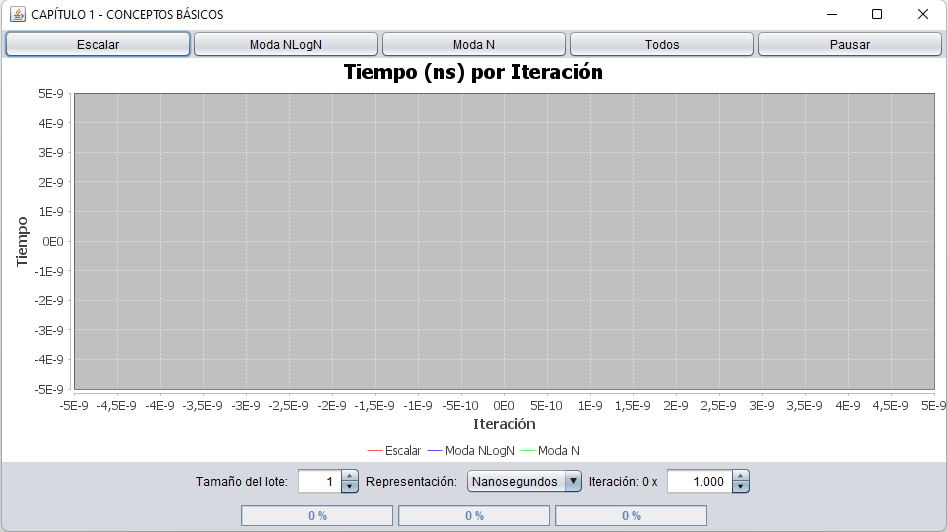
\includegraphics[width=\linewidth]{Usage/img/GUI.png}
    \caption{Interfaz de usuario}
    \label{fig:User_interface}
\end{figure}

\subsubsection{Header}
En el \say{header} de la aplicación podemos encontrar un conjunto de botones que nos permiten controlar su ejecución.\bigskip

Los cuatro primeros botones (\textit{Escalar}, \textit{Moda NLogN}, \textit{Moda N}, \textit{Todos}) ejecutan y muestra el algoritmo (o algoritmos) respectivos. Finalmente, el último botón  nos permite pausar o reanudar la ejecución actual.

\subsubsection{Main}
El principal bloque de la aplicación se encuentra el gráfico donde se representarán los tiempos de ejecución de los posibles algoritmos a ejecutar. Adicionalmente, se puede ampliar la imagen, guardarla y modificar los axis entre otros.\bigskip

Añadir que en la parte inferior del gráfico siempre se podrá consultar la leyenda, que indica que color del gráfico se relaciona a que algoritmo.

\subsubsection{Footer}
En el \say{footer} de la aplicación se pueden encontrar un conjunto de \say{gadgets} que nos permiten controlar la ejecución de los algoritmos y su visualización, además de proporcionar algo de
\say{feedback}. A continuación se explicará cada uno de ellos de izquierda a derecha:\bigskip

Primeramente, la sección definida por la etiqueta \say{Tamaño de lote} permite modificar la cantidad de llamadas a los algoritmos se harán por iteración. Si el número indicado es mayor a 1, se representará la media entre todos los resultados. \bigskip

Seguidamente, la sección definida por la etiqueta \say{Representación} permite elegir la representación temporal de los datos. Por defecto, la representación de los datos será en Nanosegundos (ns). Cuando este cambie, se actualizará tanto el nombre del gráfico como la representación de los datos, cambiando el eje x si fuese necesario. \bigskip

A su derecha, la sección definida por la etiqueta \say{Iteración} visualiza el número de iteración actual de la ejecución y su actual \say{step}. Este último aspecto permite ajustar por cuanto se quiere ponderar el número de iteración para los algoritmos. Así pues, si se tiene \texttt{5 X 500}, los algoritmos verán que se encuentran en la iteración 2500. \bigskip

Finalmente, en la parte inferior se encuentran tres barras de progreso que indican cual es el porcentaje de progreso de la ejecución actual con respecto un \texttt{timeout} definido en el código fuente. Cada una de ellas tiene asociado un color que permite identificar a que algoritmo hace referencia al ser el mismo que en la leyenda. Una vez ha llegado al 100\% la función dejará de evaluarse y se podrá tomar como finalizada.\bigskip

A continuación se muestra un ejemplo de ejecución del programa con todos los algoritmos, tamaño de lote = 1, representación en nanosegundos y 1000 de ponderación por iteración:
\begin{figure}[!h]
    \centering
    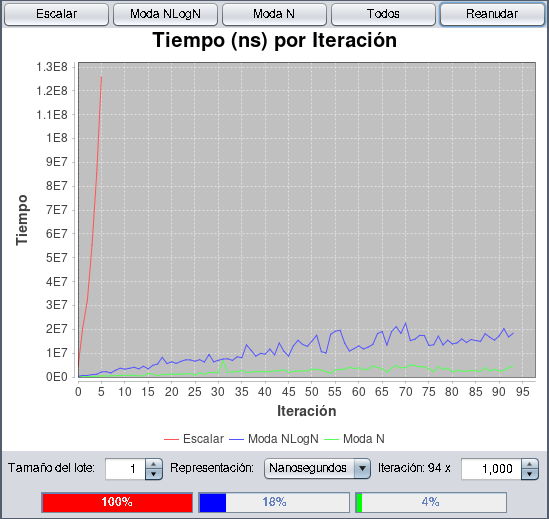
\includegraphics[width=\linewidth]{Usage/img/example_execution.png}
    \caption{Ejemplo de ejecución}
    \label{fig:example_execution}
\end{figure}